\documentclass{standalone}

\usepackage{amssymb}
\usepackage{amsmath}
\usepackage{tikz}
\usetikzlibrary{positioning}
\usetikzlibrary{arrows}

\newcommand{\R}{\mathbb{R}}
\newcommand{\D}{\mathrm{D}}

\begin{document}

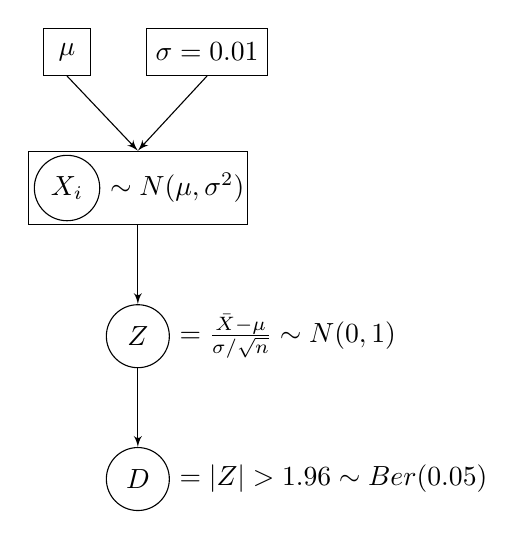
\begin{tikzpicture}[
roundnode/.style={circle, draw, minimum size=8mm},
squarenode/.style={rectangle, draw, minimum size=6mm},
vertex/.style={circle,draw,minimum size=1.5em},
edge/.style={->,> = latex'},
myblock/.style={draw}
]

%Nodes
\node[squarenode,draw=none]        (theta)                            {};
\node[squarenode]        (mu)    []         {$\mu$};
\node[squarenode]        (sigma)    [right=1]         {$\sigma=0.01$};
\node[roundnode]        (X)       [below=of theta]        {$X_i$};
\node [rectangle, draw, text width=2.55cm, text height=0.7cm, right] (Xplate) at (-0.5,-1.73) {};
\node[roundnode]        (Z)       [below=of Xplate]        {$Z$};
\node[roundnode]        (D)       [below=of Z]        {$D$};
%Node Dists
\node [rectangle, draw=none, right=0cm] (inv) at (X.east) {$\sim N(\mu, \sigma^2)$};
\node [rectangle, draw=none, right=0cm] (inv) at (Z.east) {$= \frac{\bar{X}-\mu}{\sigma / \sqrt{n}} \sim N(0, 1)$};
\node [rectangle, draw=none, right=0cm] (inv) at (D.east) {$= |Z|>1.96 \sim Ber(0.05)$};



%Edges
\draw[edge] (mu.south) -- (Xplate.north);
\draw[edge] (sigma.south) -- (Xplate.north);
\draw[edge] (Xplate.south) -- (Z.north);
\draw[edge] (Z.south) -- (D.north);
%\draw[edge] (X.south west) to[bend right] node[midway, left] {$|X-\mu| >2\sigma$} (D.north west);

%Tests Text
%\node [rectangle, draw=none] (inv) [right=3] {$\geq c(\theta_0)$?};
%\node [rectangle, draw=none] (inv)  [right=3,below=4] {$\geq c(\theta_0, \theta_1)$?};



 
    
\end{tikzpicture}

\end{document}